\documentclass[12pt]{article}
\usepackage{geometry}
\geometry{letterpaper, height=8.5in,width=6.5in}
\usepackage{graphicx}
\usepackage{amsmath}
\usepackage{amssymb}
\usepackage{pstricks}



\def\shownotes{0}  %set 1 to show author notes
\ifnum\shownotes=1
\newcommand{\authnote}[2]{$\ll$\textsf{\footnotesize #1 notes: #2}$\gg$}
\else
\newcommand{\authnote}[2]{}
\fi
\newcommand{\Tnote}[1]{{\color{blue}\authnote{Tengyu}{#1}}}

\newcommand{\commentout}[1]{}

\title{Linear Algebra Review and Reference}
\author{Zico Kolter (updated by Chuong Do and Tengyu Ma)} 

\begin{document}

\maketitle
\tableofcontents

\section{Basic Concepts and Notation}
Linear algebra provides a way of compactly representing and operating
on sets of linear equations.  For example, consider the following
system of equations:
\[\begin{array}{rcrcl} 4 x_1 & - & 5 x_2 & = & -13 \\
-2 x_1 & + & 3 x_2 & = & 9. \end{array}\\ \]

This is two equations and two variables, so as you know from high
school algebra, you can find a unique solution for $x_1$ and $x_2$ (unless
the equations are somehow degenerate, for example if the second
equation is simply a multiple of the first, but in the case above
there is in fact a unique solution).  In matrix notation, we can write
the system more compactly as
\[Ax = b\]
with 
\[A = \left [ \begin{array}{cc} 4 & -5 \\ -2 & 3
  \end{array} \right ], \quad  b = \left [ \begin{array}{c} -13 \\
    9 \end{array} \right ]. \]

As we will see shortly, there are many advantages (including the
obvious space savings) to analyzing linear equations in this form.

\subsection{Basic Notation}

We use the following notation:

\begin{itemize}

\item By $A \in \mathbb{R}^{m \times n}$ we denote a matrix with $m$ rows
  and $n$ columns, where the entries of $A$ are real numbers.

\item By $x \in \mathbb{R}^n$, we denote a vector with $n$ entries.
  By convention, an $n$-dimensional vector is often thought of as a
  matrix with $n$ rows and 1 column, known as a \textbf{\textit{column vector}}.  
  If we want to explicitly
  represent a \textbf{\textit{row vector}} --- a matrix with 1 row and
  $n$ columns --- we typically write $x^T$ (here $x^T$ denotes the
  transpose of $x$, which we will define shortly).

\item The $i$th element of a vector $x$ is denoted $x_i$: \[ x = \left
  [ \begin{array}{c} x_1 \\ x_2 \\ \vdots \\ x_n \end{array} \right
  ]. \]

\item We use the notation $a_{ij}$ (or $A_{ij}$,
  $A_{i,j}$, etc) to denote the entry of $A$ in the $i$th row
  and $j$th column: \[A = \left [ \begin{array}{cccc} a_{11} &
  a_{12} & \cdots & a_{1n} \\ a_{21} & a_{22} & \cdots & a_{2n} \\
  \vdots & \vdots & \ddots & \vdots \\ a_{m1} & a_{m2} & \cdots &
  a_{mn} \end{array} \right ].\]

\item We denote the $j$th column of $A$ by $a^j$ or $A_{:,j}$: \[ A =
  \left [ \begin{array}{cccc} | & | &  & 
  | \\ a^1 & a^2 & \cdots & a^n \\ | & | &  & |
  \end{array} \right ]. \]

\item We denote the $i$th row of $A$ by $a^T$ or $A_{i,:}$: \[ A = \left
  [ \begin{array}{ccc} \mbox{---} & a^T_1 & 
  \mbox{---} \\   \mbox{---} & a^T_2 &  \mbox{---} \\ & \vdots & \\
  \mbox{---} & a^T_m  &  \mbox{---} \end{array} \right ]. \]

\item Viewing a matrix as a collection of column or row vectors is very important and convenient in many cases. In general,  it would be mathematically (and conceptually) cleaner to operate on the level of vectors instead of scalars. There is no universal convention for denoting the columns or rows of a matrix, and thus you can feel free to change the notations as long as it's explicitly defined. %We also note that the notation here for the columns or rows of a matrix is not necessarily universally adopted, therefore 

\end{itemize}

\section{Matrix Multiplication}

The product of two matrices $A \in \mathbb{R}^{m \times n}$ and $B \in
\mathbb{R}^{n \times p}$ is the matrix \[C = AB \in \mathbb{R}^{m
  \times p},\] where \[C_{ij} = \sum_{k=1}^n A_{ik}B_{kj}.\]  Note
that in order for the matrix product to exist, the number of columns
in $A$ must equal the number of rows in $B$. There are
many other ways of looking at matrix multiplication that may be more convenient and insightful than the standard definition above, and we'll start by
examining a few special cases.

\subsection{Vector-Vector Products}

Given two vectors $x, y \in \mathbb{R}^n$, the quantity $x^T y$,
sometimes called the \textbf{\textit{inner product}} or
\textbf{\textit{dot product}} of
the vectors, is a real number given by
\[x^T y \in \mathbb{R} = 
\left [ \begin{array}{cccc} x_1 & x_2 & \cdots & x_n \end{array} \right ]
\left [ \begin{array}{c} y_1 \\ y_2 \\ \vdots \\ y_n \end{array} \right ]
= \sum_{i=1}^n x_i y_i.\]
Observe that inner products are really just special case of matrix multiplication.
Note that it is always the case that $x^T y = y^T x$.

Given vectors $x \in \mathbb{R}^m$, $y \in \mathbb{R}^n$ (not necessarily 
of the same size), $x y^T \in \mathbb{R}^{m \times n}$ is called the \textbf{\textit{outer
  product}} of the vectors.  It is a matrix whose entries are given by
$(x y^T)_{ij} = x_i y_j$, i.e.,
\[ x y^T \in \mathbb{R}^{m \times n} 
= \left [ \begin{array}{c} x_1 \\ x_2 \\ \vdots \\ x_m \end{array} \right ]
\left [ \begin{array}{cccc} y_1 & y_2 & \cdots & y_n \end{array} \right ]
= \left [ \begin{array}{cccc}x_1
    y_1 & x_1 y_2 & \cdots & x_1 
    y_n \\ x_2 y_1 & x_2 y_2 & \cdots & x_2 y_n \\ \vdots & \vdots &
    \ddots & \vdots \\ x_m y_1 & x_m y_2 & \cdots & x_m y_n
    \end{array} \right ]. \]
As an example of how the outer product can be useful, let $\mathbf{1} \in \mathbb{R}^n$
denote an $n$-dimensional vector whose entries are all equal to 1.  Furthermore,
consider the matrix $A \in \mathbb{R}^{m \times n}$ whose columns are all
equal to some vector $x \in \mathbb{R}^m$.  Using outer products, we can
represent $A$ compactly as,
\[A = \left [ \begin{array}{cccc} | & | &  & 
  | \\ x & x & \cdots & x \\ | & | &  & |
  \end{array} \right ] 
= \left [ \begin{array}{cccc}x_1
    & x_1 & \cdots & x_1 
    \\ x_2 & x_2 & \cdots & x_2 \\ \vdots & \vdots &
    \ddots & \vdots \\ x_m & x_m & \cdots & x_m 
    \end{array} \right ] 
= \left [ \begin{array}{c} x_1 \\ x_2 \\ \vdots \\ x_m \end{array} \right ]
\left [ \begin{array}{cccc} 1 & 1 & \cdots & 1 \end{array} \right ]
= x \mathbf{1}^T. \]
  

\subsection{Matrix-Vector Products}

Given a matrix $A \in \mathbb{R}^{m \times n}$ and a vector $x \in
\mathbb{R}^n$, their product is a vector $y = Ax \in \mathbb{R}^m$.
There are a couple ways of looking at matrix-vector multiplication,
and we will look at each of them in turn.

If we write $A$ by rows, then we can express $Ax$ as,
\[ y = Ax = \left [ \begin{array}{ccc} \mbox{---} & a^T_1 & 
  \mbox{---} \\   \mbox{---} & a^T_2 &  \mbox{---} \\ & \vdots & \\
  \mbox{---} & a^T_m  &  \mbox{---} \end{array} \right ] x = \left [
  \begin{array}{c} a^T_1 x \\ a^T_2 x \\ \vdots \\ a^T_m x 
  \end{array} \right ]. \]
In other words, the $i$th entry of $y$ is equal to the inner
product of the $i$th \textit{row} of $A$ and $x$, $y_i = a_i^T x$.

Alternatively, let's write $A$ in column form.  In this case we see
that,
\begin{align}
y = Ax = \left [ \begin{array}{cccc} | & | &  & 
| \\ a^1 & a^2 & \cdots & a^n \\ | & | &  & |
\end{array} \right ] \left [ \begin{array}{c} x_1 \\ x_2 \\ \vdots
\\ x_n \end{array} \right  ] = \left [ \begin{array}{c}  \\ a^1
\\  \\ \end{array} \right ] x_1 + \left [ \begin{array}{c}  \\ a^2
\\  \\ \end{array} \right ] x_2 + \ldots +  \left [ \begin{array}{c}
\\ a^n \\  \\ \end{array} \right ] x_n \;\;.  \label{eqn:2}
\end{align}


In other words, y is a \textbf{\textit{linear combination}} of the
\textit{columns} of $A$, where the coefficients of the linear
combination are given by the entries of $x$. 

So far we have been multiplying on the right by a column vector, but
it is also possible to multiply on the left by a row vector.  This is
written, $y^T = x^T A$ for $A \in \mathbb{R}^{m \times n}$, $x \in
\mathbb{R}^m$, and $y \in \mathbb{R}^n$.  As before, we can express
$y^T$ in two obvious ways, depending on whether we express $A$ in
terms on its rows or columns.  In the first case we express $A$ in
terms of its columns, which gives
\[y^T = x^T A = x^T \left [ \begin{array}{cccc} | & | &  & 
  | \\ a^1 & a^2 & \cdots & a^n \\ | & | &  & |
  \end{array} \right ] = \left [
  \begin{array}{cccc} x^T a^1 & x^T a^2 & \cdots & x^T a^n \end{array}
  \right ] \]
which demonstrates that the $i$th entry of $y^T$ is equal to the inner
product of $x$ and the $i$th \textit{column} of $A$.

Finally, expressing $A$ in terms of rows we get the final
representation of the vector-matrix product,
\begin{eqnarray*}
y^T & = & x^T A \\
    & = & \left [ \begin{array}{cccc}x_1 & x_2 & \cdots & x_n 
  \end{array} \right ] \left [ \begin{array}{ccc} \mbox{---} & a^T_1 & 
  \mbox{---} \\   \mbox{---} & a^T_2 &  \mbox{---} \\ & \vdots & \\
  \mbox{---} & a^T_m  &  \mbox{---} \end{array} \right ] \\ & & \\ 
& = & x_1 \left [ \begin{array}{ccc} \mbox{---} & a^T_1 & \mbox{---}
  \end{array} \right ] + x_2 \left [ \begin{array}{ccc} \mbox{---} &
    a^T_2 & \mbox{---} \end{array} \right ] + ... + x_n \left [
    \begin{array}{ccc} \mbox{---} & a^T_n & \mbox{---} \end{array} \right ]
\end{eqnarray*}
so we see that $y^T$ is a linear combination of the \textit{rows} of
$A$, where the coefficients for the linear combination are given by
the entries of $x$.

\subsection{Matrix-Matrix Products}\label{subsec:matrix-matrix}

Armed with this knowledge, we can now look at four different (but, of
course, equivalent) ways of
viewing the matrix-matrix multiplication $C = AB$ as defined at the
beginning of this section.  

First, we can view matrix-matrix
multiplication as a set of vector-vector products.  The most obvious
viewpoint, which follows 
immediately from the definition, is that the $(i,j)$th entry of $C$ is
equal to the inner product of the $i$th row of $A$ and the $j$th column
of $B$.  Symbolically, this looks like the following,
\[C = AB = \left [ \begin{array}{ccc} \mbox{---} & a^T_1 & 
  \mbox{---} \\   \mbox{---} & a^T_2 &  \mbox{---} \\ & \vdots & \\
  \mbox{---} & a^T_m  &  \mbox{---} \end{array} \right ] \left [
  \begin{array}{cccc} | & | &  & | \\ b^1 & b^2 & \cdots & b^p \\ | &
  | &  & | \end{array} \right ] = \left [ \begin{array}{cccc}a^T_1 b^1
    & a^T_1 b^2 & \cdots & a^T_1 b^p \\ a^T_2 b^1 & a^T_2 b^2 & \cdots &
    a^T_2 b^p \\ \vdots & \vdots & \ddots & \vdots \\ a^T_m b^1 &
    a^T_m b^2 & \cdots & a^T_m b^p \end{array} \right ]. \]
Remember that since $A \in \mathbb{R}^{m \times n}$ and $B \in
\mathbb{R}^{n \times p}$, $a_i \in \mathbb{R}^n$ and $b^j \in
\mathbb{R}^n$, so these inner products all make sense. This is the
most ``natural'' representation when we represent $A$ by 
rows and $B$ by columns.  
Alternatively, we can represent $A$ by
columns, and $B$ by rows.  This representation leads to a much trickier interpretation of $AB$ as
a sum of outer products.  Symbolically,
\[C = AB = \left [ \begin{array}{cccc} | & | &  & | \\ a^1 & a^2 &
    \cdots & a^n \\ | & | &  & | \end{array} \right ] \left [
  \begin{array}{ccc} \mbox{---} & b^T_1 & \mbox{---} \\   \mbox{---} &
    b^T_2 &  \mbox{---} \\ & \vdots & \\ \mbox{---} & b^T_n  &
    \mbox{---} \end{array} \right ] = \sum_{i=1}^n a^i
    b_i^T \;\;.\]
Put another way, $AB$ is equal to the sum, over all $i$, of the outer
product of the $i$th 
column of $A$ and the $i$th row of $B$.  Since, in this case, $a^i \in
\mathbb{R}^m$ and $b_i \in \mathbb{R}^p$, the dimension of the
outer product $a^i b^T_i$ is $m \times p$, which coincides with the
dimension of $C$.  Chances are, the last equality above may appear 
confusing to you.  If so, take the time to check it for yourself!

Second, we can also view matrix-matrix multiplication as a set of
matrix-vector products. Specifically, if we represent $B$ by columns,
we can view the columns of $C$ as matrix-vector products between $A$
and the columns of $B$.  Symbolically,
\begin{align}
C = AB = A \left [ \begin{array}{cccc} | & | &  & | \\ b^1 & b^2 &
    \cdots & b^p \\ | & | &  & | \end{array} \right ] = \left [
    \begin{array}{cccc} | & | &  & | \\ A b^1 & A b^2 & \cdots & A b^p \\ |
      & | &  & | \end{array} \right ]. \label{eqn:1}
\end{align}
Here the $i$th column of $C$ is given by the matrix-vector product
with the vector on the right, $c_i = A b_i$.  These matrix-vector
products can in turn be interpreted using both viewpoints given in the
previous subsection.  Finally, we have the analogous viewpoint, where
we represent $A$ by rows, and view the rows of $C$ as the
matrix-vector product between the rows of $A$ and $C$.  Symbolically,
\[C = AB = \left [ \begin{array}{ccc} \mbox{---} & a^T_1 & 
  \mbox{---} \\   \mbox{---} & a^T_2 &  \mbox{---} \\ & \vdots & \\
  \mbox{---} & a^T_m  &  \mbox{---} \end{array} \right ] B = \left [
  \begin{array}{ccc} \mbox{---} & a^T_1 B &  \mbox{---} \\   \mbox{---}
  & a^T_2 B &  \mbox{---} \\ & \vdots & \\ 
  \mbox{---} & a^T_m B  &  \mbox{---} \end{array} \right ]. \]
Here the $i$th row of $C$ is given by the matrix-vector product with
the vector on the left, $c_i^T = a_i^T B$.

It may seem like overkill to dissect matrix multiplication to such a
large degree, especially when all these viewpoints follow immediately
from the initial definition we gave (in about a line of math) at the
beginning of this section. {\bf The direct advantage of these various viewpoints is that they allow you to operate on the level/unit of vectors instead of scalars.} To fully understand linear algebra without getting lost in the complicated manipulation of indices, the key is to operate with as large concepts as possible. \footnote{E.g., if you could write all your math derivations with matrices or vectors, it would be better than doing them with scalar elements.}
\Tnote{I am not sure what's the best way to write this philosophical remark about doing math.. Any better idea?}

Virtually all of linear algebra
deals with matrix multiplications of some kind, and it is worthwhile
to spend some time trying to develop an intuitive understanding of the
viewpoints presented here.

In addition to this, it is useful to know a few basic properties of
matrix multiplication at a higher level:
\begin{itemize}
\item Matrix multiplication is associative: $(AB)C = A(BC)$.
\item Matrix multiplication is distributive: $A(B + C) = AB + AC$.
\item Matrix multiplication is, in general, \textit{not} commutative;
  that is, it can be the case that $AB \neq BA$.  (For example,
  if $A \in \mathbb{R}^{m \times n}$ and $B \in \mathbb{R}^{n \times q}$,
  the matrix product $BA$ does not even exist if $m$ and $q$ are not equal!)
\end{itemize}

If you are not familiar with these properties, take the time to verify 
them for yourself.  For example, to check the associativity of matrix
multiplication, suppose that $A \in \mathbb{R}^{m \times n}$, 
$B \in \mathbb{R}^{n \times p}$, and $C \in \mathbb{R}^{p \times q}$.  
Note that $AB \in \mathbb{R}^{m \times p}$, so $(AB)C \in \mathbb{R}^{m \times q}$.
Similarly, $BC \in \mathbb{R}^{n \times q}$, so $A(BC) \in \mathbb{R}^{m \times q}$.
Thus, the dimensions of the resulting matrices agree.  To show that
matrix multiplication is associative, it suffices to check that the $(i,j)$th
entry of $(AB)C$ is equal to the $(i,j)$th entry of $A(BC)$.  We can verify 
this directly using the definition of matrix multiplication:
\begin{eqnarray*}
((AB)C)_{ij} &=& \sum_{k=1}^p (AB)_{ik}C_{kj} = \sum_{k=1}^p \left(\sum_{l=1}^n A_{il} B_{lk}\right) C_{kj} \\
&=& \sum_{k=1}^p \left(\sum_{l=1}^n A_{il} B_{lk} C_{kj} \right) = \sum_{l=1}^n \left(\sum_{k=1}^p A_{il} B_{lk} C_{kj} \right) \\
&=& \sum_{l=1}^n A_{il} \left(\sum_{k=1}^p B_{lk} C_{kj}\right) = \sum_{l=1}^n A_{il} (BC)_{lj} = (A(BC))_{ij}.
\end{eqnarray*}
Here, the first and last two equalities simply use the definition of matrix multiplication,
the third and fifth equalities use the distributive property for \textit{scalar multiplication over addition}, and
the fourth equality uses the \textit{commutative and associativity of scalar addition}.  This technique for proving
matrix properties by reduction to simple scalar properties will come up often, so make sure you're familiar with it.

\section{Operations and Properties}

In this section we present several operations and properties of
matrices and vectors. Hopefully a great deal of this will be review
for you, so the notes can just serve as a reference for these topics.

\subsection{The Identity Matrix and Diagonal Matrices}
The \textbf{\textit{identity matrix}}, denoted $I \in \mathbb{R}^{n
  \times n}$, is a square matrix with ones on the diagonal and zeros
  everywhere else.  That is,
\[ I_{ij} = \left \{ \begin{array}{ll}1 & i = j \\ 0 & i \neq j
  \end{array} \right . \]
It has the property that for all $A \in \mathbb{R}^{m \times n}$, \[AI
= A = IA.\]   Note that in some sense, the notation for the identity matrix
is ambiguous, since it does not specify the dimension of $I$.  Generally, 
the dimensions of $I$ are inferred from context so as to make matrix multiplication
possible.  For example, in the
equation above, the $I$ in $AI = A$ is an $n \times n$ matrix, whereas
the $I$ in $A = IA$ is an $m \times m$ matrix.

A \textbf{\textit{diagonal matrix}} is a matrix where all non-diagonal
elements are 0.  This is typically denoted $D = \mathrm{diag}(d_1,
d_2, \ldots, d_n)$, with
\[ D_{ij} = \left \{ \begin{array}{ll}d_i & i = j \\ 0 & i \neq
  j\end{array} \right . \]
Clearly, $I = \mathrm{diag}(1,1,\ldots,1)$.

\subsection{The Transpose}
The \textbf{\textit{transpose}} of a matrix results from ``flipping''
the rows and columns.  Given a matrix $A \in \mathbb{R}^{m \times n}$,
its transpose, written $A^T \in \mathbb{R}^{n \times m}$, is the $n \times m$ matrix
whose entries are given by
\[ (A^T)_{ij} = A_{ji}.\]
We have in fact already been using the transpose when describing row
vectors, since the transpose of a column vector is naturally a row
vector.

The following properties of transposes are easily verified:
\begin{itemize}
\item $(A^T)^T = A$
\item $(AB)^T = B^T A^T$
\item $(A + B)^T = A^T + B^T$
\end{itemize}

\subsection{Symmetric Matrices}
A square matrix $A \in \mathbb{R}^{n \times n}$ is
\textbf{\textit{symmetric}} if $A = A^T$.  It is
\textbf{\textit{anti-symmetric}} if $A = -A^T$.  It is easy to show
that for any matrix $A \in \mathbb{R}^{n \times n}$, the matrix
$A + A^T$ is symmetric and the matrix $A - A^T$ is anti-symmetric.
From this it follows that any square matrix $A \in \mathbb{R}^{n
  \times n}$ can be represented as a sum of a symmetric matrix and an
anti-symmetric matrix, since
\[A = \frac{1}{2}(A + A^T) + \frac{1}{2}(A - A^T)\]
and the first matrix on the right is symmetric, while the second is
anti-symmetric.  It turns out that symmetric matrices occur a great
deal in practice, and they have many nice properties which we will
look at shortly.  It is common to denote the set of all symmetric
matrices of size $n$ as $\mathbb{S}^n$, so that $A \in \mathbb{S}^n$
means that $A$ is a symmetric $n \times n$ matrix;

\subsection{The Trace}
The \textbf{\textit{trace}} of a square matrix $A \in \mathbb{R}^{n
  \times n}$, denoted $\mathrm{tr}(A)$ (or just $\mathrm{tr}A$ if the
  parentheses are obviously implied), is the
sum of diagonal elements in the matrix: 
\[\mathrm{tr}A = \sum_{i=1}^n A_{ii}.\]
As described in the CS229 lecture notes, the trace has the following
properties (included here for the sake of completeness):
\begin{itemize}
\item For $A \in \mathbb{R}^{n \times n}$, $\mathrm{tr}A =
  \mathrm{tr}A^T$.
\item For $A,B \in \mathbb{R}^{n \times n}$, $\mathrm{tr}(A + B) =
  \mathrm{tr}A + \mathrm{tr}B$.
\item For $A \in \mathbb{R}^{n \times n}$, $t \in \mathbb{R}$,
  $\mathrm{tr}(tA) = t \; \mathrm{tr}A$.
\item For $A,B$ such that $AB$ is square, $\mathrm{tr}AB =
  \mathrm{tr}BA$.
\item For $A,B,C$ such that $ABC$ is square, $\mathrm{tr}ABC =
  \mathrm{tr}BCA = \mathrm{tr}CAB$, and so on for the product of
  more matrices.
\end{itemize}

As an example of how these properties can be proven, we'll consider the
fourth property given above.  Suppose that $A \in \mathbb{R}^{m \times n}$
and $B \in \mathbb{R}^{n \times m}$ (so that $AB \in \mathbb{R}^{m \times m}$ is a square matrix).
Observe that $BA \in \mathbb{R}^{n \times n}$ is also a square matrix, so it makes sense
to apply the trace operator to it.  To verify that $\mathrm{tr} AB = \mathrm{tr} BA$, note that
\begin{eqnarray*}
  \mathrm{tr} AB &=& \sum_{i=1}^m (AB)_{ii} = \sum_{i=1}^m \left(\sum_{j=1}^n A_{ij} B_{ji} \right) \\
  &=& \sum_{i=1}^m \sum_{j=1}^n A_{ij} B_{ji} = \sum_{j=1}^n \sum_{i=1}^m B_{ji} A_{ij} \\
  &=& \sum_{j=1}^n \left(\sum_{i=1}^m B_{ji} A_{ij}\right) = \sum_{j=1}^n (BA)_{jj} = \mathrm{tr} BA.
\end{eqnarray*}
Here, the first and last two equalities use the definition of the trace operator and matrix multiplication.
The fourth equality, where the main work occurs, uses the commutativity of scalar multiplication in order
to reverse the order of the terms in each product, and the commutativity and associativity of scalar addition
in order to rearrange the order of the summation.

\commentout{
As an example of how these properties can be proven, we'll consider the last
property given above.  Suppose that $A \in \mathbb{R}^{m \times n}$, 
$B \in \mathbb{R}^{n \times p}$, and $C \in \mathbb{R}^{p \times m}$ (so that $ABC \in \mathbb{R}^{m \times m}$ is a square matrix).
In this case, it is easy to see that $BCA \in \mathbb{R}^{n \times n}$ is also
a square matrix.  To verify that $\mathrm{tr}ABC = \mathrm{tr}BCA$, observe that
\begin{eqnarray*}
  \mathrm{tr} ABC &=& \sum_{i=1}^m (ABC)_{ii} = \sum_{i=1}^m \left(\sum_{j=1}^p (AB)_{ij} C_{ji} \right) = \sum_{i=1}^m \left(\sum_{j=1}^p \left( \sum_{k=1}^n A_{ik} B_{kj} \right) C_{ji} \right) \\
  &=& \sum_{i=1}^m \sum_{j=1}^p \sum_{k=1}^n A_{ik} B_{kj} C_{ji} = \sum_{k=1}^n \sum_{i=1}^m \sum_{j=1}^p B_{kj} C_{ji} A_{ik} \\
  &=& \sum_{k=1}^n \sum_{i=1}^m \left( \sum_{j=1}^p B_{kj} C_{ji} \right) A_{ik} = \sum_{k=1}^n \sum_{i=1}^m (BC)_{ki} A_{ik} \\
  &=& \sum_{k=1}^n (BCA)_{kk} = \mathrm{tr} BCA.
\end{eqnarray*}
}

\subsection{Norms}

A \textbf{\textit{norm}} of a vector $\|x\|$ is informally a measure of
the ``length'' of the vector.  For example, we have the 
commonly-used Euclidean or $\ell_2$ norm,
\[\|x\|_2 = \sqrt{\sum_{i=1}^n x_i^2}.\]
Note that $\|x\|_2^2 = x^Tx$.

More formally, a norm is any function $f : \mathbb{R}^{n} \rightarrow
\mathbb{R}$ that satisfies 4 properties:
\begin{enumerate}
\item For all $x \in \mathbb{R}^n$, $f(x) \geq 0$ (non-negativity).
\item $f(x) = 0$ if and only if $x = 0$ (definiteness).
\item For all $x \in \mathbb{R}^n$, $t \in \mathbb{R}$, $f(tx) =
  |t|f(x)$ (homogeneity).
\item For all $x,y \in \mathbb{R}^n$, $f(x + y) \leq f(x) + f(y)$
  (triangle inequality).
\end{enumerate}
Other examples of norms are the $\ell_1$ norm,
\[\|x\|_1 = \sum_{i=1}^n |x_i| \]
and the $\ell_\infty$ norm,
\[\|x\|_\infty = \mathrm{max}_i\, |x_i|.\]
In fact, all three norms presented so far are examples of the family
of $\ell_p$ norms, which are parameterized by a real number $p \geq
1$, and defined as
\[\|x\|_p = \left ( \sum_{i=1}^n |x_i|^p \right )^{1/p}.\]

Norms can also be defined for matrices, such as the Frobenius norm,
\[\|A\|_F = \sqrt{\sum_{i=1}^m \sum_{j=1}^n A_{ij}^2} =
\sqrt{\mathrm{tr}(A^T A)}. \] Many other norms exist, but they are
beyond the scope of this review.

\subsection{Linear Independence and Rank}
A set of vectors $\{x_1, x_2, \ldots x_n\} \subset \mathbb{R}^m\ $ is said to be
\textbf{\textit{(linearly) independent}} if no vector can be represented
as a linear combination of the remaining vectors.  Conversely, if one
vector belonging to the set \textit{can} be represented as a linear combination of
the remaining vectors, then the vectors are said to be \textbf{\textit{(linearly)
    dependent}}.  That is, if
\[x_n = \sum_{i=1}^{n-1} \alpha_i x_i\]
for some scalar values $\alpha_1, \ldots, \alpha_{n-1} \in \mathbb{R}$, then we say that
the vectors $x_1, \ldots, x_n$ are linearly dependent; otherwise, the vectors are
linearly independent.  For example, the vectors
\[
x_1 = \left[ \begin{array}{c} 1 \\ 2 \\ 3 \end{array} \right] \quad 
x_2 = \left[ \begin{array}{c} 4 \\ 1 \\ 5 \end{array} \right] \quad 
x_3 = \left[ \begin{array}{c} 2 \\ -3 \\ -1 \end{array} \right] 
\]
are linearly dependent because $x_3 = -2x_1 + x_2$.

The \textbf{\textit{column rank}} of a matrix $A \in \mathbb{R}^{m \times n}$ is the 
size of the largest subset of columns of $A$ that constitute a linearly independent
set.  With some abuse of terminology, this is often referred to simply as the number of linearly
independent columns of $A$.  In the same way, the
\textbf{\textit{row rank}} is the largest number of rows of $A$ that
constitute a linearly independent set.

For any matrix $A \in \mathbb{R}^{m \times n}$, it turns out that
the column rank of $A$ is equal to the row rank of $A$ (though we will not prove this), and so both quantities
are referred to collectively as the \textbf{\textit{rank}} of $A$, denoted as
$\mathrm{rank}(A)$.  The following are some basic properties of the
rank: 
\begin{itemize}
\item For $A \in \mathbb{R}^{m \times n}$, $\mathrm{rank}(A) \leq
    \mathrm{min}(m,n)$.  If $\mathrm{rank}(A) = \mathrm{min}(m,n)$,
    then $A$ is said to be \textbf{\textit{full rank}}. 
  \item For $A \in \mathbb{R}^{m \times n}$, $\mathrm{rank}(A) =
    \mathrm{rank}(A^T)$.
  \item For $A \in \mathbb{R}^{m \times n}$, $B \in \mathbb{R}^{n
    \times p}$, $\mathrm{rank}(AB) \leq \mathrm{min}(\mathrm{rank}(A),
    \mathrm{rank}(B))$.
  \item For $A,B \in \mathbb{R}^{m \times n}$, $\mathrm{rank}(A + B)
    \leq \mathrm{rank}(A) + \mathrm{rank}(B)$.
\end{itemize}

\subsection{The Inverse of a Square Matrix}

The \textbf{\textit{inverse}} of a square matrix $A \in \mathbb{R}^{n
  \times n}$ is denoted $A^{-1}$, and is the unique matrix such that
\[A^{-1} A = I = A A^{-1}.\]  
Note that not all matrices have inverses.  Non-square matrices, for example,
do not have inverses by definition.  However, for some square matrices
$A$, it may still be the case that $A^{-1}$ may not exist.  In particular,
we say that $A$ is \textbf{\textit{invertible}} or
\textbf{\textit{non-singular}} if $A^{-1}$ exists and
\textbf{\textit{non-invertible}} or \textbf{\textit{singular}}
otherwise.\footnote{It's easy to get confused and think that non-singular means non-invertible.  But in fact, it means the opposite!  Watch out!}  

In order for a square matrix $A$ to have an inverse $A^{-1}$, then
$A$ must be full rank.  We will soon see that there are many
alternative sufficient and necessary conditions, in addition to full
rank, for invertibility.  

The following are properties of the inverse;
all assume that $A, B \in \mathbb{R}^{n \times n}$ are non-singular:
\begin{itemize}
\item $(A^{-1})^{-1} = A$
\item $(AB)^{-1} = B^{-1} A^{-1}$
\item $(A^{-1})^T = (A^T)^{-1}$.  For this reason this matrix is often
  denoted $A^{-T}$.
\end{itemize}
As an example of how the inverse is used, consider the linear system of equations,
$Ax = b$ where $A \in \mathbb{R}^{n \times n}$, and $x, b \in \mathbb{R}^n$.  If
$A$ is nonsingular (i.e., invertible), then $x = A^{-1} b$.   

(What if $A \in \mathbb{R}^{m \times n}$
is not a square matrix?  Does this work?)

\Tnote{Add more about pseudo-inverse}

\subsection{Orthogonal Matrices}
Two vectors $x,y \in \mathbb{R}^n$ are \textbf{\textit{orthogonal}} if
$x^T y$ = 0. A vector $x \in \mathbb{R}^n$ is
\textbf{\textit{normalized}} if $\|x\|_2 = 1$.  A square matrix $U \in
\mathbb{R}^{n \times n}$ is \textbf{\textit{orthogonal}} (note the
different meanings when talking about vectors versus matrices) if all
its columns are orthogonal to each other and are normalized (the
columns are then referred to as being \textbf{\textit{orthonormal}}).

It follows immediately from the definition of orthogonality and
normality that
\[U^TU = I = UU^T.\]
In other words, the inverse of an orthogonal matrix is its transpose.
Note that if $U$ is not square --- i.e., $U \in \mathbb{R}^{m \times
  n},\;\; n < m$ --- but its columns are still orthonormal, then $U^TU
= I$, but $U U^T \neq I$.  We generally only use the term orthogonal
to describe the previous case, where $U$ is square.

Another nice property of orthogonal matrices is that operating on a
vector with an orthogonal matrix will not change its Euclidean norm,
i.e.,
\begin{align}
\|Ux\|_2 = \|x\|_2 \label{eqn:preserve-norm}
\end{align}
for any $x \in \mathbb{R}^n$, $U \in \mathbb{R}^{n \times n}$
orthogonal.

\subsection{Range and Nullspace of a Matrix}
The \textbf{\textit{span}} of a set of vectors $\{x_1, x_2, \ldots
x_n\}$ is the set of all vectors that can be expressed as a linear
combination of $\{x_1, \ldots, x_n\}$.  That is,
\[\mathrm{span}(\{x_1, \ldots x_n\}) = \left \{v : v = \sum_{i=1}^n \alpha_i
x_i, \;\; \alpha_i \in
\mathbb{R} \right \}. \]
It can be shown that if $\{x_1, \ldots, x_n\}$ is a set of $n$
linearly independent vectors, where each $x_i \in \mathbb{R}^n$, then
$\mathrm{span}(\{x_1, \ldots x_n\}) = \mathbb{R}^n$.  In other words,
\textit{any} vector $v \in \mathbb{R}^n$ can be written as a linear
combination of $x_1$ through $x_n$.  The
\textbf{\textit{projection}} of a vector $y \in \mathbb{R}^m$ onto the
span of $\{x_1, \ldots, x_n\}$ (here we assume
$x_i \in \mathbb{R}^m$) is the
vector $v \in \mathrm{span}(\{x_1, \ldots x_n\})$, such that $v$ is as
close as possible to $y$, 
as measured by the Euclidean norm $\|v - y\|_2$.  We denote the
projection as $\mathrm{Proj}(y;\{x_1, \ldots, x_n\})$ and can define
it formally as,
\[\mathrm{Proj}(y;\{x_1, \ldots x_n\}) = \textrm{argmin}_{v \in
  \mathrm{span}(\{x_1, \ldots, x_n\})} \|y - v\|_2.\]  

The \textbf{\textit{range}} (sometimes also called the columnspace)
of a matrix $A \in \mathbb{R}^{m \times n}$, denoted $\mathcal{R}(A)$,
is the the span of the columns of $A$.  In other words, 
\[\mathcal{R}(A) = \{v \in \mathbb{R}^m: v = Ax, x \in
\mathbb{R}^{n}\}.\]  Making a 
few technical assumptions (namely that $A$ is full rank and that $n <
m$), the projection of a vector $y \in \mathbb{R}^m$ onto the range of
$A$ is given by,
\[\mathrm{Proj}(y;A) = \mathrm{argmin}_{v \in \mathcal{R}(A)} \|v -
y\|_2 = A (A^T A)^{-1}A^T y\;\;.\]  This last equation should look
extremely familiar, since it is almost the same formula we derived in
class (and which we will soon derive again)
for the least squares estimation of parameters.  Looking at the
definition for the projection, it should not be too hard to convince
yourself that this is in fact the same objective that we minimized in
our least squares problem (except for a squaring of the norm, which
doesn't affect the optimal point) and so these problems are naturally
very connected.  When $A$ contains only a single column, $a \in
\mathbb{R}^m$, this gives the special case for a projection of a
vector on to a line: 
\[\mathrm{Proj}(y;a) = \frac{a a^T}{a^T a}y\;\;.\]

The \textbf{\textit{nullspace}} of a matrix $A \in \mathbb{R}^{m
  \times n}$, denoted $\mathcal{N}(A)$ is the set of all
  vectors that equal 0 when multiplied by $A$, i.e.,
\[\mathcal{N}(A) = \{x \in \mathbb{R}^n : Ax = 0\}.\]  Note that
vectors in $\mathcal{R}(A)$ are of size $m$, while vectors in the
$\mathcal{N}(A)$ are of size $n$, so vectors in $\mathcal{R}(A^T)$
and $\mathcal{N}(A)$ are both in $\mathbb{R}^n$.  In fact, we can
say much more.  It turns out that 
\[\left \{ w : w = u + v, u \in \mathcal{R}(A^T), v \in \mathcal{N}(A)
  \right \}  = \mathbb{R}^n \mbox{  and
} \mathcal{R}(A^T) \cap \mathcal{N}(A) = \{\mathbf{0}\}\;\;.\]
In other words, $\mathcal{R}(A^T)$ and $\mathcal{N}(A)$ are disjoint
subsets that together span the entire space of $\mathbb{R}^n$.  Sets
of this type are called \textbf{\textit{orthogonal complements}}, and
we denote this $\mathcal{R}(A^T) = \mathcal{N}(A)^\perp$.

\subsection{The Determinant}
The \textbf{\textit{determinant}} of a square matrix $A \in
\mathbb{R}^{n \times n}$, is a function $\mathrm{det} : \mathbb{R}^{n
  \times n} \rightarrow \mathbb{R}$, and is denoted $|A|$ or $\mathrm{det}\,A$
(like the trace operator, we usually omit parentheses).  
Algebraically,
one could write down an explicit formula for the determinant of $A$, but
this unfortunately gives little intuition about its meaning.  Instead,
we'll start out by providing a geometric interpretation of the determinant
and then visit some of its specific algebraic properties afterwards.

Given a matrix
\[ \left [ \begin{array}{ccc} \mbox{---} & a^T_1 & 
    \mbox{---} \\   \mbox{---} & a^T_2 &  \mbox{---} \\ & \vdots & \\
  \mbox{---} & a^T_n  &  \mbox{---} \end{array} \right ], \] 
consider the set of points $S \subset \mathbb{R}^n$ formed by taking
all possible linear combinations of the row vectors $a_1, \ldots, a_n \in \mathbb{R}^n$ of $A$,
where the coefficients of the linear combination are all between 0 and 1;
that is, the set $S$ is the restriction of $\textrm{span}(\{a_1,\ldots,a_n\})$
to only those linear combinations whose coefficients $\alpha_1, \ldots, \alpha_n$ 
satisfy $0 \le \alpha_i \le 1$, $i=1,\ldots,n$.  Formally,
\[ S = \{ v \in \mathbb{R}^n : v = \sum_{i=1}^n \alpha_i a_i \mbox{ where } 0 \le \alpha_i \le 1, i=1,\ldots,n \}. \]
The absolute value of the determinant of $A$, it turns out, is a measure of the ``volume'' of the set $S$.\footnote{
  Admittedly, we have not actually defined what we mean by ``volume'' here, but hopefully the intuition should be clear enough.
  When $n=2$, our notion of ``volume'' corresponds to the area of $S$ in the Cartesian plane.  When $n=3$, ``volume'' corresponds
  with our usual notion of volume for a three-dimensional object.
}

For example, consider the $2 \times 2$ matrix,
\begin{equation}
  A = \left[ \begin{array}{cc} 1 & 3 \\ 3 & 2 \end{array} \right]. \label{eq:det-example} 
\end{equation}
Here, the rows of the matrix are
\[ a_1 = \left[ \begin{array}{c} 1 \\ 3 \end{array} \right] \quad a_2 = \left[ \begin{array}{c} 3 \\ 2 \end{array} \right]. \]
The set $S$ corresponding to these rows is shown in Figure~\ref{fig:determinant}.  For two-dimensional matrices,
$S$ generally has the shape of a \emph{parallelogram}.  In our example, the value of the determinant is $|A| = -7$ (as can be computed
using the formulas shown later in this section), so the area of the parallelogram is $7$.  (Verify this for yourself!)

In three dimensions, the set $S$ corresponds to an object known as a \emph{parallelepiped} (a three-dimensional box with skewed sides, such that
every face has the shape of a parallelogram).  The absolute value of the determinant of the $3 \times 3$ matrix whose rows define $S$ give
the three-dimensional volume of the parallelepiped.  In even higher dimensions, the set $S$ is an object known as an $n$-dimensional \emph{parallelotope}.
%

%\begin{figure}
%  \vskip 5.0cm
%  \psline[linewidth=0.05]{->}(6,0)(11,0)
%  \psline[linewidth=0.05]{->}(6,0)(6,5)
%  \pspolygon[linewidth=0.05,fillstyle=solid,fillcolor=lightgray](6,0)(7,3)(10,5)(9,2)
%  \rput(6.3,1.9){$a_1$}
%  \rput(8,0.8){$a_2$}
%  \psline[linewidth=0.1]{->}(6,0)(7,3)
%  \psline[linewidth=0.1]{->}(6,0)(9,2)
%  \rput(6.5,3.2){$(1,3)$}
%  \rput(9.5,1.9){$(3,2)$}
%  \rput(10.2,5.4){$(4,5)$}
%  \rput(5.4,0){$(0,0)$}
%  \caption{
%    Illustration of the determinant for the $2 \times 2$ matrix $A$ given in \eqref{eq:det-example}.  Here, $a_1$ and $a_2$ are vectors
%    corresponding to the rows of $A$, and the set $S$ corresponds to the shaded region (i.e., the parallelogram).  The
%    absolute value of the determinant, $|\textrm{det} A| = 7$, is the area of the parallelogram. 
%  }
%  \label{fig:determinant}
%\end{figure}

\begin{figure}[t]
  \begin{center}
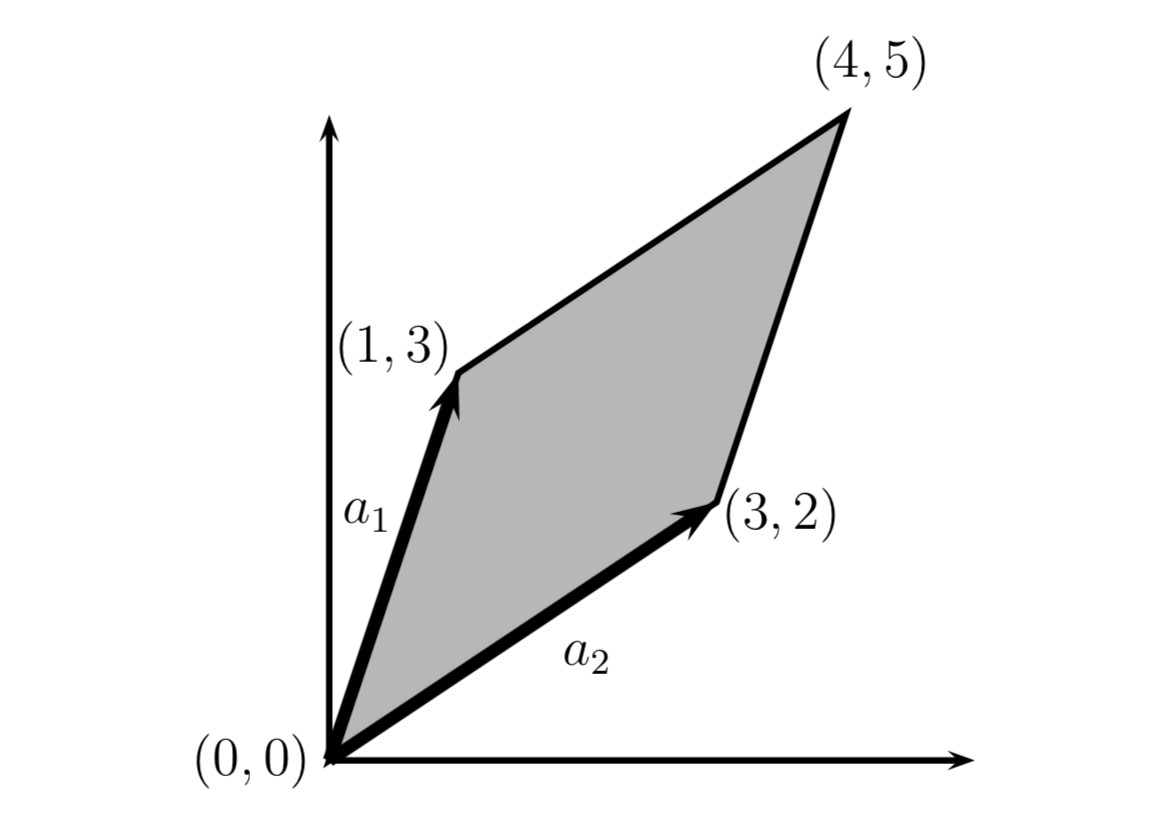
\includegraphics[width=0.6\textwidth]{figures/figure}
  \caption{
    Illustration of the determinant for the $2 \times 2$ matrix $A$ given in \eqref{eq:det-example}.  Here, $a_1$ and $a_2$ are vectors
    corresponding to the rows of $A$, and the set $S$ corresponds to the shaded region (i.e., the parallelogram).  The
    absolute value of the determinant, $|\textrm{det} A| = 7$, is the area of the parallelogram. 
  }
  \end{center}
  \label{fig:determinant}
\end{figure}

Algebraically, the determinant satisfies the following three properties (from which all other properties follow, including the
general formula):
\begin{enumerate}
\item The determinant of the identity is 1, $|I| = 1$.  (Geometrically, the volume of a unit hypercube is 1).   
\item Given a matrix $A \in \mathbb{R}^{n \times n}$, if we multiply a
  single row in $A$ by a scalar $t \in \mathbb{R}$, then the
  determinant of the new matrix is $t |A|$,
\[\left | \left [ \begin{array}{ccc} \mbox{---} & t \; a^T_1 & 
  \mbox{---} \\   \mbox{---} & a^T_2 &  \mbox{---} \\ & \vdots & \\
  \mbox{---} & a^T_m  &  \mbox{---} \end{array} \right ] \right |= t
  |A|. \] 
  (Geometrically, multiplying one of the sides of the set $S$ by a factor $t$
  causes the volume to increase by a factor $t$.)
\item If we exchange any two rows $a_i^T$ and $a_j^T$ of $A$, then the
  determinant of the new matrix is $-|A|$, for example
\[\left | \left [ \begin{array}{ccc} \mbox{---} & a^T_2 & 
  \mbox{---} \\   \mbox{---} & a^T_1 &  \mbox{---} \\ & \vdots & \\
  \mbox{---} & a^T_m  &  \mbox{---} \end{array} \right ] \right |=
  -|A|. \]  
\end{enumerate}
In case you are wondering, it is not immediately obvious that a function satisfying
the above three properties exists.  In fact, though, such a function does exist, 
and is unique (which we will not prove here).  

Several properties that follow from the three properties above include:
\begin{itemize}
\item For $A \in \mathbb{R}^{n \times n}$, $|A| = |A^T|$.
\item For $A, B \in \mathbb{R}^{n \times n}$, $|AB| = |A||B|$.
\item For $A \in \mathbb{R}^{n \times n}$, $|A| = 0$ if and only if
  $A$ is singular (i.e., non-invertible).
  (If $A$ is singular then it does not have full rank, and hence
  its columns are linearly dependent.  In this case, the set $S$ corresponds to a
  ``flat sheet'' within the $n$-dimensional space and hence has zero volume.)
\item For $A \in \mathbb{R}^{n \times n}$ and $A$ non-singular,
  $|A^{-1}| = 1/|A|$.
\end{itemize}

Before giving the general definition for the determinant, we define,
for $A \in \mathbb{R}^{n \times n}$, $A_{\setminus i,\setminus j} \in
\mathbb{R}^{(n-1) \times (n-1)}$ to be the \textit{matrix} that
results from deleting the $i$th row and $j$th column from $A$.  The
general (recursive) formula for the determinant is
\begin{eqnarray*}
|A| & = & \sum_{i=1}^n (-1)^{i+j} a_{ij} |A_{\setminus i, \setminus
  j}| \;\;\;\;\;\mbox{(for any $j \in 1,\ldots, n$)} \\
& = & \sum_{j=1}^n (-1)^{i+j} a_{ij} |A_{\setminus i, \setminus j}|
  \;\;\;\;\;\mbox{(for any $i \in 1,\ldots, n$)}
\end{eqnarray*}
with the initial case that $|A| = a_{11}$ for $ A \in
\mathbb{R}^{1 \times 1}$.   If we were to expand this formula
completely for $A \in \mathbb{R}^{n \times n}$, there would be a total
of $n!$ ($n$ factorial) different terms.  For this reason, we hardly
ever explicitly write the complete equation of the determinant for
matrices bigger than $3 \times 3$.  However, the equations for
determinants of matrices up to size $3 \times 3$ are fairly common,
and it is good to know them:
\begin{eqnarray*}
\left | [a_{11}] \right | & = & a_{11} \\
\left | \left [ \begin{array}{cc} a_{11} & a_{12} \\ a_{21} & a_{22}
  \end{array} \right ] \right | & = & a_{11} a_{22} - a_{12} a_{21} \\
\left | \left [ \begin{array}{ccc} a_{11} & a_{12} & a_{13} \\ a_{21}
    & a_{22} & a_{23} \\ a_{31} & a_{32} & a_{33} \end{array} \right ]
    \right | & = &\begin{array}{l} a_{11} a_{22} a_{33} + a_{12} a_{23} a_{31} +
    a_{13} a_{21} a_{32} \\ \;\;\;\;\; - a_{11} a_{23} a_{32} - a_{12}
    a_{21} a_{33} - a_{13} a_{22} a_{31} \end{array}
\end{eqnarray*}

The \textbf{\textit{classical adjoint}} (often just called the
adjoint) of a matrix $A \in \mathbb{R}^{n \times n}$, is denoted
$\mathrm{adj}(A)$, and defined as
\[\mathrm{adj}(A) \in \mathbb{R}^{n \times n}, \;\;\;
(\mathrm{adj}(A))_{ij} = (-1)^{i+j} |A_{\setminus j, \setminus
  i}|\;\;\]
(note the switch in the indices $A_{\setminus j, \setminus i}$).  It
  can be shown that for any nonsingular $A \in \mathbb{R}^{n \times 
  n}$,
\[A^{-1} = \frac{1}{|A|}\mathrm{adj}(A)\;\;.\]
While this is a nice ``explicit'' formula for the inverse of matrix,
we should note that, numerically, there are in fact much more
efficient ways of computing the inverse.

\subsection{Quadratic Forms and Positive Semidefinite Matrices}
Given a square matrix $A \in \mathbb{R}^{n \times n}$ and a vector $x
\in \mathbb{R}^n$, the scalar value $x^T A x$ is called a
\textbf{\textit{quadratic form}}.  Written explicitly, we see that
\[x^T A x = \sum_{i=1}^n x_i (Ax)_i = \sum_{i=1}^n x_i \left(\sum_{j=1}^n A_{ij} x_j\right) = \sum_{i=1}^n \sum_{j=1}^n A_{ij} x_i x_j\;\;.\]
Note that,
\[x^T A x = (x^T A x)^T = x^T A^T x = x^T\left(\frac{1}{2} A +
\frac{1}{2}A^T\right)x,\]
where the first equality follows from the fact that the transpose
of a scalar is equal to itself, and the second equality follows
from the fact that we are averaging two quantities which are themselves equal.
From this, we can conclude that 
only the symmetric part of $A$ contributes to the quadratic
form.  For this reason, we often implicitly assume that the matrices
appearing in a quadratic form are symmetric.

We give the following definitions:
\begin{itemize}
\item A symmetric matrix $A \in \mathbb{S}^n$ is
\textbf{\textit{positive definite}} (PD) if for all non-zero
vectors $x \in \mathbb{R}^n$, $x^T A x > 0$.  This is usually
denoted $A \succ 0$ (or just $A > 0$), and often times the set of
all positive definite matrices is denoted $\mathbb{S}^n_{++}$. 
  

\item A symmetric matrix $A \in \mathbb{S}^n$ is
\textbf{\textit{positive semidefinite}} (PSD) if for all vectors
$x^T A x \geq 0$.  This is written $A \succeq 0$ (or just $A \geq
0$), and the set of all positive semidefinite matrices is often
denoted $\mathbb{S}^n_+$.

\item Likewise, a symmetric matrix $A \in
\mathbb{S}^n$ is \textbf{\textit{negative definite}} (ND), denoted $A
\prec 0$ (or just $A < 0$) if for all non-zero $x \in
\mathbb{R}^n$, $x^T A x < 0$.

\item Similarly, a symmetric matrix $A \in \mathbb{S}^n$ is
    \textbf{\textit{negative semidefinite}} (NSD), denoted $A \preceq
    0$ (or just $A \leq 0$) if for all $x \in \mathbb{R}^n$, $x^T A x 
\leq 0$.

\item Finally, a symmetric matrix $A \in
\mathbb{S}^n$ is \textbf{\textit{indefinite}}, if it is neither
positive semidefinite nor negative semidefinite --- i.e., if there
exists $x_1, x_2 \in \mathbb{R}^n$ such that $x_1^T A x_1 > 0$ and
$x_2^T A x_2 < 0$.

\end{itemize}

It should be obvious that if $A$ is positive definite, then $-A$ is
negative definite and vice versa.  Likewise, if $A$ is positive
semidefinite then $-A$ is negative semidefinite and vice versa.  If
$A$ is indefinite, then so is $-A$.  

One important property of positive definite and negative definite matrices 
is that they are always full rank, and hence, invertible.  To see why
this is the case, suppose that some matrix $A \in \mathbb{R}^{n \times n}$
is not full rank.  Then, suppose that the $j$th column of $A$ is expressible 
as a linear combination of other $n-1$ columns:
\[ a_j = \sum_{i \neq j} x_i a_i, \]
for some $x_1,\ldots,x_{j-1}, x_{j+1}, \ldots,x_{n} \in \mathbb{R}$.  Setting $x_j = -1$, we have
\[ Ax = \sum_{i=1}^n x_i a_i = 0. \]
But this implies $x^T Ax = 0$ for some non-zero vector $x$, so $A$ must be
neither positive definite nor negative definite.  Therefore, if $A$ is
either positive definite or negative definite, it must be full rank.

Finally, there is one type of positive definite matrix that comes up
frequently, and so deserves some special mention.  Given any matrix $A
\in \mathbb{R}^{m \times n}$ (not necessarily symmetric or even
square), the matrix $G = A^T A$ (sometimes called a
\textbf{\textit{Gram matrix}}) is always positive semidefinite.
Further, if $m \geq n$ (and we assume for convenience that $A$ is full
rank), then $G = A^T A$ is positive definite.

\subsection{Eigenvalues and Eigenvectors}

Given a square matrix $A \in \mathbb{R}^{n \times n}$, we say that
$\lambda \in \mathbb{C}$ is an \textbf{\textit{eigenvalue}} of $A$ and
$x \in \mathbb{C}^n$  is the corresponding
\textbf{\textit{eigenvector}}\footnote{Note that $\lambda$ and the
  entries of $x$ are actually in 
$\mathbb{C}$, the set of complex numbers, not just the reals; we
will see shortly why this is necessary. Don't worry about this
technicality for now, you can think of complex vectors in the same way
as real vectors.} if
\[Ax = \lambda x, \;\;\; x \neq 0. \]
Intuitively, this definition
means that multiplying $A$ by the vector $x$ results in a new vector
that points in the same direction as $x$, but scaled by a factor
$\lambda$.  Also note that for any eigenvector $x \in \mathbb{C}^n$,
and scalar $t \in \mathbb{C}$, 
$A(cx) = cAx = c \lambda x = \lambda(cx)$, so $cx$ is also an
eigenvector.   For this reason when we talk about ``the'' eigenvector
associated with $\lambda$, we usually assume that the eigenvector is
normalized to have length 1 (this still creates some ambiguity, since
$x$ and $-x$ will both be eigenvectors, but we will have to live with
this).

We can rewrite the equation above to state that $(\lambda, x)$ is an
eigenvalue-eigenvector pair of $A$ if,
\[(\lambda I - A)x = 0, \;\;\; x \neq 0.\]
But $(\lambda I - A)x = 0$ has a non-zero solution to $x$ if and only
if $(\lambda I - A)$ has a non-empty nullspace, which is only the case
if $(\lambda I - A)$ is singular, i.e.,
\[|(\lambda I - A)| = 0.\]


We can now use the previous definition of the determinant to expand
this expression $|(\lambda I - A)|$ into a (very large) polynomial in $\lambda$, where
$\lambda$ will have  degree $n$. It's often called the characteristic polynomial of the matrix $A$. 

We then find the $n$
(possibly complex) roots of this characteristic polynomial and denote them by $\lambda_1, \ldots, \lambda_n$. These are all the eigenvalues of the matrix $A$, but we note that they may not be distinct. 
To find the eigenvector
corresponding to the eigenvalue $\lambda_i$, we simply solve the
linear equation $(\lambda_i I - A)x = 0$, which is guaranteed to have a non-zero solution because $\lambda_i I-A$ is singular (but there could also be multiple or infinite solutions.)




It should be noted that
this is not the method which is actually used in practice to
numerically compute the eigenvalues and eigenvectors (remember that
the complete expansion of the determinant has $n!$ terms); it is
rather a mathematical argument.  

The following are properties of
eigenvalues and eigenvectors (in all cases assume $A \in \mathbb{R}^{n
  \times n}$ has eigenvalues $\lambda_i, \ldots, \lambda_n$):
\begin{itemize}
\item The trace of a $A$ is equal to the sum of its eigenvalues,
\[\mathrm{tr}A = \sum_{i=1}^n \lambda_i.\]
\item The determinant of $A$ is equal to the product of its
  eigenvalues,
\[|A| = \prod_{i=1}^n \lambda_i.\]
\item The rank of $A$ is equal to the number of non-zero eigenvalues
  of $A$.
\item Suppose $A$ is non-singular with eigenvalue $\lambda$ and an associated eigenvector $x$. Then $1/\lambda$ is an eigenvalue of
  $A^{-1}$ with an associated eigenvector $x$, i.e., $A^{-1}x =
  (1/\lambda)x$.  (To prove this, take the eigenvector equation,
  $A x = \lambda x$ and left-multiply each side by $A^{-1}$.)
\item The eigenvalues of a diagonal matrix $D = \mathrm{diag}(d_1,
  \ldots d_n)$ are just the diagonal entries $d_1, \ldots d_n$.
\end{itemize}
%We can write all the eigenvector equations simultaneously as
%\[AX = X\Lambda\]
%where the columns of $X \in \mathbb{R}^{n \times n}$ are the
%eigenvectors of $A$ and $\Lambda$ is a diagonal matrix whose entries
%are the eigenvalues of $A$, i.e.,
%\[X \in \mathbb{R}^{n \times n} = \left [\begin{array}{cccc} | & | &
%    & | \\ x_1 & x_2 & \cdots & x_n \\ | &  | &  & | \end{array}
%  \right ], \;\; \Lambda  =
%  \mathrm{diag}(\lambda_1, \ldots, \lambda_n).\]
%If the eigenvectors of $A$ are linearly independent, then the matrix
%$X$ will be invertible, so $A = X\Lambda X^{-1}$.  A matrix that can
%be written in this form is called \textbf{\textit{diagonalizable}}.


\subsection{Eigenvalues and Eigenvectors of Symmetric Matrices}


In general, the structures of the eigenvalues and eigenvectors of a general square matrix can be subtle to characterize. Fortunately, in most of the cases in machine learning, it suffices to deal with symmetric real matrices, whose eigenvalues and eigenvectors have remarkable properties. 


%Two remarkable properties come about when we look at the eigenvalues
%and eigenvectors of a symmetric matrix $A \in \mathbb{S}^n$.  


Throughout this section, let's assume that $A$ is a symmetric real matrix. We have the following properties: 

\begin{itemize}
	\item[1.] All eigenvalues of $A$ are real numbers. We denote them by $\lambda_1,\dots, \lambda_n$. 
	\item[2.] There exists a set of eigenvectors $u_1,\dots, u_n$ such that a) for all $i$, $u_i$ is an eigenvector with eigenvalue $\lambda_i$ and b) $u_1,\dots, u_n$ are unit vectors and orthogonal to each other.\footnote{Mathematically, we have $\forall i,  Au_i = \lambda_i u_i$, $\|u_i\|_2=1$, and $\forall j\neq i, u_i^Tu_j=0$. Moreover, we remark that it's not true that all eigenvectors $u_1,\dots, u_n$ satisfying a) of any matrix $A$ are orthogonal to each other, because the eigenvalues can be repetitive and so can eigenvectors.}
\end{itemize}

Let $U$ be the orthonormal matrix that contains $u_i$'s as columns:\footnote{Here for notational simplicity, we deviate from the notational convention for columns of matrices in the previous sections.}

\begin{align}
U = \left [
\begin{array}{cccc} | & | &  & | \\ u_1 & u_2 & \cdots & u_n \\ | &
| &  & | \end{array} \right ]
\end{align}

Let $\Lambda  =
\mathrm{diag}(\lambda_1, \ldots, \lambda_n)$ be the diagonal matrix that contains $\lambda_1,\dots, \lambda_n$ as entries on the diagonal. Using the view of matrix-matrix vector multiplication in equation~\eqref{eqn:1} of Section~\ref{subsec:matrix-matrix}, we can verify that 
\begin{align}
AU & =  \left [
\begin{array}{cccc} | & | &  & | \\A u_1 & Au_2 & \cdots & Au_n \\ | &
| &  & | \end{array} \right ] =  \left [
\begin{array}{cccc} | & | &  & | \\ \lambda_1 u_1 & \lambda_2 u_2 & \cdots & \lambda_n u_n \\ | &
| &  & | \end{array} \right ]  = U\mathrm{diag}(\lambda_1, \ldots, \lambda_n) = U\Lambda \nonumber
\end{align}

Recalling that orthonormal matrix $U$ satisfies that $UU^T = I$ and using the equation above, we have 
\begin{align}
A = AUU^T = U\Lambda U^T \label{eqn:3}
\end{align}

This new presentation of $A$ as $U\Lambda U^T$ is often called the diagonalization of the matrix $A$. The term diagonalization comes from the fact that with such representation, we can often effectively treat a symmetric matrix $A$ as a diagonal matrix --- which is much easier to understand --- w.r.t the basis defined by the eigenvectors $U$. We will elaborate this below by several examples. 

\newcommand{\R}{\mathbb{R}}
\paragraph{Background: representing vector w.r.t. another basis.} Any orthonormal matrix $U =  \left [
\begin{array}{cccc} | & | &  & | \\ u_1 &  u_2 & \cdots & u_n \\ | &
| &  & | \end{array} \right ]  $ defines a new basis (coordinate system) of $\mathbb{R}^n$ in the following sense. For any vector $x\in \mathbb{R}^n$ can be represented as a linear combination of $u_1,\dots, u_n$ with coefficient $\hat{x}_1,\dots, \hat{x}_n$:
\begin{align}
x = \hat{x}_1 u_1 + \dots + \hat{x}_n u_n  = U\hat{x} \nonumber
\end{align}
where in the second equality we use the view of equation~\eqref{eqn:2}. Indeed, such $\hat{x}$ uniquely exists 
\begin{align}
x = U\hat{x} \Leftrightarrow U^T x = \hat{x} \nonumber
\end{align}
In other words,  the vector $\hat{x}= U^T x$ can serve as another representation of the vector $x$ w.r.t the basis defined by $U$. 


\paragraph{``Diagonalizing'' matrix-vector multiplication.} With the setup above, we will see that left-multiplying matrix $A$ can be viewed as left-multiplying a diagonal matrix w.r.t the basic of the eigenvectors. Suppose $x$ is a vector and $\hat{x}$ is its representation w.r.t to the basis of $U$. Let $z = Ax$ be the matrix-vector product. Now let's compute the representation $z$ w.r.t the basis of $U$: 

Then, again using the fact that $UU^T = U^TU = I$ and equation~\eqref{eqn:3},  we have that 
\begin{align}
\hat{z} = U^T z = U^T Ax = U^T U\Lambda U^T x = \Lambda \hat{x}  = \left [ \begin{array}{c} \lambda_1 \hat{x}_1 \\ \lambda_2 \hat{x}_2 \\ \vdots \\ \lambda_n \hat{x}_n  \end{array} \right ]\nonumber
\end{align}
We see that left-multiplying matrix $A$ in the original space is equivalent to left-multiplying the diagonal matrix $\Lambda$ w.r.t the new basis, which is merely scaling each coordinate by the corresponding eigenvalue. %One of the key features here is that under the new basis, all the coordinates are scaled independently.  

Under the new basis, multiplying a matrix multiple times becomes much simpler as well. For example, suppose $q = AAAx$. Deriving out the analytical form of $q$ in terms of the entries of $A$ may be a nightmare under the original basis, but can be much easier under the new on: 
\begin{align}
\hat{q} = U^T q = U^TAx = U^TU\Lambda U^TU\Lambda U^TU\Lambda U^Tx = \Lambda^3 \hat{x} = \left [ \begin{array}{c} \lambda_1^3 \hat{x}_1 \\ \lambda_2^3 \hat{x}_2 \\ \vdots \\ \lambda_n^3 \hat{x}_n  \end{array} \right ]
\end{align}








%First, it can be shown that all the eigenvalues of $A$ are real.  


%Secondly,
%the eigenvectors of $A$ are orthonormal, i.e., the matrix $X$ defined
%$above is an orthogonal matrix (for this reason, we denote the matrix
%f eigenvectors as $U$ in this case). 

%
%We can therefore represent $A$
%as $A = U\Lambda U^T$, remembering from above that the inverse of an
%orthogonal matrix is just its transpose.

\paragraph{``Diagonalizing'' quadratic form.} As a directly corollary, the quadratic form $x^TAx$ can also be simplified under the new basis
\begin{align}
x^TAx = x^TU\Lambda U^T x = \hat{x} \Lambda \hat{x} = \sum_{i=1}^n \lambda_i\hat{x}_i^2 \label{eqn:diag-quadratic}
\end{align}
(Recall that with the old representation, $x^TAx = \sum_{i=1,j=1}^{n} x_ix_jA_{ij}$ involves a sum of $n^2$ terms instead of $n$ terms in the equation above.) With this viewpoint,  we can also show that the definiteness of the matrix $A$ depends
entirely on the sign of its eigenvalues:
\begin{itemize}
	\item[1.]   If all $\lambda_i > 0$, then the matrix $A$ s positivedefinite because $x^TAx = \sum_{i=1}^n \lambda_i\hat{x}_i^2 > 0$ for any $\hat{x}\neq 0$.\footnote{Note that $\hat{x}\neq 0\Leftrightarrow x\neq 0$.} 
	\item[2.]  If all $\lambda_i \geq 0$, it is positive semidefinite because $x^TAx = \sum_{i=1}^n \lambda_i\hat{x}_i^2 \ge  0$ for all $\hat{x}$. 
	\item[3.]  Likewise, if all $\lambda_i < 0$ or $\lambda_i \leq 0$, then $A$ is
	negative definite or negative semidefinite respectively.  
	\item[4.] Finally, if
	$A$ has both positive and negative eigenvalues, say $\lambda_i > 0$ and $\lambda_j < 0$, then it is indefinite. This is because if we let $\hat{x}$ satisfy $\hat{x}_i = 1 $ and $\hat{x}_k =0, \forall k\neq i$, then $x^TAx = \sum_{i=1}^n \lambda_i\hat{x}_i^2 > 0$. Similarly we can let $\hat{x}$ satisfy $\hat{x}_j = 1 $ and $\hat{x}_k =0, \forall k\neq j$, then $x^TAx = \sum_{i=1}^n \lambda_i\hat{x}_i^2  < 0$. \footnote{Note that $x = U\hat{x}$ and therefore constructing $\hat{x}$ gives an implicit construction of $x$. }
\end{itemize}
  %Suppose $A \in \mathbb{S}^n
%= U \Lambda U^T$.  
%
%Then
%\[x^T A x = x^T U \Lambda U^T x = y^T \Lambda y = \sum_{i=1}^n
%%\lambda_i y_i^2\]
%where $y = U^T x$ (and since $U$ is full rank, any vector $y \in
%\mathbb{R}^n$ can be represented in this form).  Because $y_i^2$ is
%always positive, the sign of this expression depends entirely on the
%$\lambda_i$'s.  If all $\lambda_i > 0$, then the matrix is positive
%definite; if all $\lambda_i \geq 0$, it is positive semidefinite.
%Likewise, if all $\lambda_i < 0$ or $\lambda_i \leq 0$, then $A$ is
%negative definite or negative semidefinite respectively.  Finally, if
%$A$ has both positive and negative eigenvalues, it is indefinite.

An application where eigenvalues and eigenvectors come up frequently
is in maximizing some function of a matrix.  In particular, for a
matrix $A \in \mathbb{S}^n$, consider the following maximization
problem, 
\begin{align}\mathrm{max}_{x \in \mathbb{R}^n} \;\; x^T A x = \sum_{i=1}^n \lambda_i\hat{x}_i^2  \;\;\;\;\;
\mbox{subject to } \|x\|_2^2 = 1\label{eqn:4}
\end{align}
i.e., we want to find the vector (of norm 1) which maximizes the
quadratic form.  Assuming the eigenvalues are ordered as $\lambda_1
\geq \lambda_2 \geq \ldots \geq \lambda_n$, the optimal value of this optimization problem is $\lambda_1$ and any eigenvector $u_1$ corresponding to $\lambda_1$ is one of the maximizers. (If $\lambda_1 > \lambda_2$, then there is a unique eigenvector corresponding to eigenvalue $\lambda_1$, which is the unique maximizer of the optimization problem~\eqref{eqn:4}.)

We can show this by using the diagonalization technique: Note that $\|x\|_2 = \|\hat{x}\|_2$ by equation~\eqref{eqn:preserve-norm}, and using equation~\eqref{eqn:diag-quadratic}, we can rewrite the optimization~\eqref{eqn:4} as
\begin{align}
\mathrm{max}_{\hat{x} \in \mathbb{R}^n} \;\; \hat{x}^T \Lambda \hat{x} = \sum_{i=1}^n \lambda_i\hat{x}_i^2 \;\;\;\;\;
\mbox{subject to } \|\hat{x}\|_2^2 = 1\label{eqn:5}
\end{align}

%the optimal $x$ for this
%optimization problem is $x_1$, the eigenvector corresponding to
%$\lambda_1$.  In this case the maximal value of the quadratic form is
%$\lambda_1$.  Similarly, the optimal solution to the minimization
%%problem,
%\[\mathrm{min}_{x \in \mathbb{R}^n} \;\; x^T A x \;\;\;\;\;
%\mbox{subject to } \|x\|_2^2 = 1\]

Then, we have that the objective is upper bounded by $\lambda_1$:
\begin{align}
\hat{x}^T \Lambda \hat{x} = \sum_{i=1}^n \lambda_i\hat{x}_i^2 \le \sum_{i=1}^n \lambda_1 \hat{x}_i^2  = \lambda_1
\end{align}
Moreover, setting $\hat{x} = \left [ \begin{array}{c} 1 \\ 0\\ \vdots \\ 0  \end{array} \right ]$ achieves the equality in the equation above, and this corresponds to setting $x = u_1$. 

%
%is $x_n$, the eigenvector corresponding to $\lambda_n$, and the
%minimal value is $\lambda_n$.  This can be proved by appealing to the 
%eigenvector-eigenvalue form of $A$ and the properties of orthogonal
%matrices.  However, in the next section we will see a way of showing
%it directly using matrix calculus.


\section{Matrix Calculus}
While the topics in the previous sections are typically covered in a
standard course on linear algebra, one topic that does not seem to be
covered very often (and which we will use extensively) is the
extension of calculus to the vector setting.  Despite the fact that
all the actual calculus we use is relatively trivial, the notation can
often make things look much more difficult than they are.  In this
section we present some basic definitions of matrix calculus and
provide a few examples.

\subsection{The Gradient}
Suppose that $f:\mathbb{R}^{m \times n} \rightarrow \mathbb{R}$ is a
function that takes as input a matrix $A$ of size $m \times n$ and
returns a real value.  Then the \textbf{\textit{gradient}} of $f$
(with respect to $A \in \mathbb{R}^{m \times n}$) is the matrix of
partial derivatives, defined as:
\[\nabla_A f(A) \in \mathbb{R}^{m \times n} = \left [
  \begin{array}{cccc} \frac{\partial f(A)}{\partial A_{11}} & 
  \frac{\partial f(A)}{\partial A_{12}} & \cdots & \frac{\partial
  f(A)}{\partial A_{1n}}  \\ \frac{\partial f(A)}{\partial A_{21}} &
  \frac{\partial f(A)}{\partial A_{22}}  & \cdots & \frac{\partial
  f(A)}{\partial A_{2n}}  \\
  \vdots & \vdots & \ddots & \vdots \\ \frac{\partial f(A)}{\partial
  A_{m1}}  & \frac{\partial f(A)}{\partial A_{m2}}  & \cdots &
  \frac{\partial f(A)}{\partial A_{mn}} \end{array} \right ] \]
i.e., an $m \times n$ matrix with \[(\nabla_A f(A))_{ij} =
  \frac{\partial f(A)}{\partial A_{ij}}.\]
Note that the size of $\nabla_A f(A)$ is always the
  same as the size of $A$.  So if, in particular, $A$ is just a vector
  $x \in \mathbb{R}^n$,
\[\nabla_x f(x) = \left [ \begin{array}{c} \frac{\partial
  f(x)}{\partial x_1} \\ \frac{\partial f(x)}{\partial x_2} \\ \vdots
  \\ \frac{\partial f(x)}{\partial x_n}\end{array} \right ].\]
It is very important to remember that the gradient of a function is
\textit{only} defined if the function is real-valued, that is, if it
returns a scalar value.  We can not, for example, take the gradient of
$Ax, A \in \mathbb{R}^{n \times n}$ with respect to $x$, since this
quantity is vector-valued.

It follows directly from the equivalent properties of partial
derivatives that:
\begin{itemize}
\item $\nabla_x (f(x) + g(x)) = \nabla_x f(x) + \nabla_x g(x)$.
\item For $t \in \mathbb{R}$, $\nabla_x (t\;f(x)) = t \nabla_x f(x)$.
\end{itemize}

In principle, gradients are a natural extension of partial derivatives
to functions of multiple variables.  In practice, however, working with
gradients can sometimes be tricky for notational reasons.  
For example,
suppose that $A \in \mathbb{R}^{m \times n}$ is a matrix of fixed coefficients and 
suppose that $b \in \mathbb{R}^m$ is a vector of fixed coefficients.
Let $f : \mathbb{R}^{m} \rightarrow \mathbb{R}$ be the function defined by
$f(z) = z^T z$, such that $\nabla_z f(z) = 2z$.
But now, consider the expression,
\[ \nabla f(Ax). \]
How should this expression be interpreted?  There are at least two possibilities:
\begin{enumerate}
\item 
  In the first interpretation, recall that $\nabla_z f(z) = 2z$.  Here, we
  interpret $\nabla f(Ax)$ as evaluating the gradient at the point $Ax$, 
  hence, 
  \[ \nabla f(Ax) = 2(Ax) = 2Ax \in \mathbb{R}^m. \]
\item
  In the second interpretation, we consider the quantity $f(Ax)$ as a function of the
  input variables $x$.  More formally, let $g(x) = f(Ax)$.  Then in this interpretation,
  \[ \nabla f(Ax) = \nabla_x g(x) \in \mathbb{R}^n. \]
\end{enumerate}
Here, we can see that these two interpretations are indeed different.  One interpretation
yields an $m$-dimensional vector as a result, while the other interpretation yields an
$n$-dimensional vector as a result!  How can we resolve this?

Here, the key is to make explicit the variables which we are differentiating with respect to.
In the first case, we are differentiating the function $f$ with respect to its arguments $z$
and then substituting the argument $Ax$.  In the second case, we are differentiating the
composite function $g(x) = f(Ax)$ with respect to $x$ directly.  We denote the first
case as $\nabla_z f(Ax)$ and the second case as $\nabla_x f(Ax)$.\footnote{A drawback to this notation
that we will have to live with is the fact that in the first case, $\nabla_z f(Ax)$ it appears
that we are differentiating with respect to a variable that does not even appear in the expression
being differentiated!  For this reason, the first case is often written as $\nabla f(Ax)$, and the fact
that we are differentiating with respect to the arguments of $f$ is understood.  However,
the second case is \emph{always} written as $\nabla_x f(Ax)$.}
Keeping the notation
clear is extremely important (as you'll find out in your homework, in fact!).  

\subsection{The Hessian}
Suppose that $f:\mathbb{R}^n \rightarrow \mathbb{R}$ is a function
that takes a vector in $\mathbb{R}^n$ and returns a real number.  Then
the \textbf{\textit{Hessian}} matrix with respect to $x$, written
$\nabla_x^2 f(x)$ or simply as $H$ is the $n \times n$ matrix of
partial derivatives, 
\[\nabla^2_x f(x) \in \mathbb{R}^{n \times n} = \left [
  \begin{array}{cccc} \frac{\partial^2 f(x)}{\partial x_1^2} & 
  \frac{\partial^2 f(x)}{\partial x_1 \partial x_2} & \cdots &
  \frac{\partial^2 f(x)}{\partial x_1 \partial x_n}  \\
  \frac{\partial^2 f(x)}{\partial x_2 \partial x_1} & 
  \frac{\partial^2 f(x)}{\partial x_2^2}  & \cdots & \frac{\partial^2
  f(x)}{\partial x_2 \partial x_n}  \\
  \vdots & \vdots & \ddots & \vdots \\ \frac{\partial^2 f(x)}{\partial
  x_n \partial x_1}  & \frac{\partial^2 f(x)}{\partial x_n \partial
  x_2} & \cdots & \frac{\partial^2 f(x)}{\partial x_n^2}
  \end{array} \right ].\]
In other words, $\nabla_x^2 f(x) \in \mathbb{R}^{n \times n}$, with
\[(\nabla^2_x f(x))_{ij} = \frac{\partial^2 f(x)}{\partial x_i
  \partial x_j}.\]
Note that the Hessian is always symmetric, since
\[\frac{\partial^2 f(x)}{\partial x_i \partial x_j} = \frac{\partial^2
  f(x)}{\partial x_j \partial x_i}.\]
Similar to the gradient, the Hessian is defined only when $f(x)$ is
real-valued.  

It is natural to think of the gradient as the analogue
of the first derivative for functions of vectors, and the Hessian as
the analogue of the second derivative (and the symbols we use also
suggest this relation).  This intuition is generally
correct, but there a few caveats to keep in mind.


First, for real-valued functions of one variable $f:\mathbb{R}
  \rightarrow \mathbb{R}$, it is a basic definition that the second
  derivative is the derivative of the first derivative, i.e.,
\[\frac{\partial^2 f(x)}{\partial x^2} = \frac{\partial}{\partial x}
  \frac{\partial}{\partial x} f(x).\]
However, for functions of a vector, the gradient of the function is a
vector, and we cannot take the gradient of a vector --- i.e.,
\[\nabla_x \nabla_x f(x) = \nabla_x \left [ \begin{array}{c} \frac{\partial
  f(x)}{\partial x_1} \\ \frac{\partial f(x)}{\partial x_2} \\ \vdots
  \\ \frac{\partial f(x)}{\partial x_n}\end{array} \right ]\]
and this expression is not defined.  Therefore, it is \textit{not} the
  case that the Hessian is the gradient of the gradient.  However,
  this is \textit{almost} true, in the following sense:  If we look at
  the $i$th entry of the gradient $(\nabla_x f(x))_i = \partial f(x) /
  \partial x_i$, and take the gradient with respect to $x$ we get
\[\nabla_x \frac{\partial f(x)}{\partial x_i} = \left [
  \begin{array}{c} \frac{\partial^2 f(x)}{\partial x_i \partial x_1}
  \\ \frac{\partial^2 f(x)}{\partial x_i \partial x_2} \\ \vdots \\
  \frac{\partial f(x)}{\partial x_i \partial x_n}\end{array} \right ] \]
which is the $i$th column (or row) of the Hessian.  Therefore,
\[\nabla_x^2 f(x) = \left [ \begin{array}{cccc} \nabla_x (\nabla_x
  f(x))_1 & \nabla_x (\nabla_x f(x))_2 & 
    \cdots & \nabla_x (\nabla_x f(x))_n \end{array} \right ].\]
If we don't mind being a little bit sloppy we can say that
(essentially) $\nabla_x^2 f(x) = \nabla_x (\nabla_x f(x))^T$, so long
as we understand that this really means taking the gradient of each
entry of $(\nabla_x f(x))^T$, not the gradient of the whole vector.

Finally, note that while we can take the gradient with respect to a
matrix $A \in \mathbb{R}^n$, for the purposes of this class we will
only consider taking the Hessian with respect to a vector $x \in
\mathbb{R}^n$.  This is simply a matter of convenience (and the fact
that none of the calculations we do require us to find the Hessian
with respect to a matrix), since the Hessian with respect to a matrix
would have to represent all the partial derivatives $\partial^2 f(A) /
(\partial A_{ij} \partial A_{k\ell})$, and it is rather cumbersome to
represent this as a matrix.

\subsection{Gradients and Hessians of Quadratic and Linear Functions}

Now let's try to determine the gradient and Hessian matrices for a few
simple functions.  It should be noted that all the gradients given
here are special cases of the gradients given in the CS229 lecture
notes.  

For $x \in \mathbb{R}^n$, let $f(x) = b^T x$ for some known
vector $b \in \mathbb{R}^n$.  Then  
\[f(x) = \sum_{i = 1}^n b_i x_i\]
so
\[\frac{\partial f(x)}{\partial x_k} = \frac{\partial}{\partial x_k}
  \sum_{i = 1}^n b_i x_i = b_k.\]
From this we can easily see that $\nabla_x b^T x = b$.  This should be
compared to the analogous situation in single variable calculus, where
$\partial/(\partial x) \; ax = a$.

Now consider the quadratic function $f(x) = x^T A x$ for $A \in
\mathbb{S}^n$.  Remember that
\[f(x) = \sum_{i=1}^n \sum_{j=1}^n A_{ij} x_i x_j. \]
To take the partial derivative, we'll consider the terms including $x_k$
and $x_k^2$ factors separately:
\begin{eqnarray*}
  \frac{\partial f(x)}{\partial x_k} 
  &=& \frac{\partial}{\partial x_k} \sum_{i=1}^n \sum_{j=1}^n A_{ij} x_i x_j \\
  &=& \frac{\partial}{\partial x_k} \left[ \sum_{i \neq k} \sum_{j \neq k} A_{ij} x_i x_j + \sum_{i \neq k} A_{ik} x_i x_k + \sum_{j \neq k} A_{kj} x_k x_j + A_{kk} x_k^2 \right] \\
  &=& \sum_{i \neq k} A_{ik} x_i + \sum_{j \neq k} A_{kj} x_j + 2 A_{kk} x_k \\
  &=& \sum_{i=1}^n A_{ik} x_i + \sum_{j=1}^n A_{kj} x_j = 2 \sum_{i=1}^n A_{ki} x_i,
\end{eqnarray*}
where the last equality follows since $A$ is symmetric (which we can
safely assume, since it is appearing in a quadratic form).
Note that the $k$th entry of $\nabla_x f(x)$ is just the inner
product of the $k$th row of $A$ and $x$.  Therefore, $\nabla_x x^T A
x = 2Ax$. Again, this should remind you of the analogous fact in
single-variable calculus, that $\partial/(\partial x)\; ax^2 = 2ax$.

Finally, let's look at the Hessian of the quadratic function $f(x) =
x^T A x$ (it should be obvious that the Hessian of a linear function
$b^T x$ is zero).  In this case,
\[\frac{\partial^2 f(x)}{\partial x_k \partial x_\ell} =
\frac{\partial}{\partial x_k} \left[ \frac{\partial f(x)}{\partial x_\ell} \right] =
\frac{\partial}{\partial x_k} \left[ 2 \sum_{i=1}^n A_{\ell i} x_i \right] = 2 A_{\ell k} = 2 A_{k \ell}.\]
Therefore, it should be clear that $\nabla_x^2 x^T A x = 2 A$, which
should be entirely expected (and again analogous to the
single-variable fact that $\partial^2/(\partial x^2)\;ax^2 = 2a$).

To recap,
\begin{itemize}
\item $\nabla_x b^T x = b$
\item $\nabla_x x^T A x = 2Ax$ (if $A$ symmetric)
\item $\nabla_x^2 x^T A x = 2A$ (if $A$ symmetric)
\end{itemize}

\subsection{Least Squares}

Let's apply the equations we obtained in the last section to
derive the least squares equations.  Suppose we are given matrices $A
\in \mathbb{R}^{m \times n}$ (for simplicity we assume $A$ is full
rank) and a vector $b \in \mathbb{R}^m$ such that $b \not \in
\mathcal{R}(A)$.  In this situation we will not be able to find a
vector $x \in \mathbb{R}^n$, such that $Ax = b$, so instead we want to
find a vector $x$ such that $Ax$ is as close as possible to $b$, as
measured by the square of the Euclidean norm $\|Ax - b\|_2^2$.

Using the fact that $\|x\|_2^2$ = $x^T x$, we have
\begin{eqnarray*}
\|Ax - b\|_2^2 & = & (Ax - b)^T(Ax - b) \\
& = & x^T A^T A x - 2b^T Ax + b^T b
\end{eqnarray*}
Taking the gradient with respect to $x$ we have, and using the
properties we derived in the previous section
\begin{eqnarray*}
\nabla_x (x^T A^T A x - 2b^T Ax + b^T b) & = & \nabla_x x^T A^T A x -
\nabla_x 2b^T Ax + \nabla_x b^T b \\
& = & 2 A^T A x - 2 A^T b
\end{eqnarray*}
Setting this last expression equal to zero and solving for $x$ gives
the normal equations 
\[x = (A^T A)^{-1}A^T b\]
which is the same as what we derived in class.

\subsection{Gradients of the Determinant}
Now let's consider a situation where we find the gradient of a function
with respect to a matrix, namely for $A \in \mathbb{R}^{n \times n}$,
we want to find $\nabla_A |A|$.  Recall from our discussion of
determinants that
\[ |A| = \sum_{i=1}^n (-1)^{i+j} A_{ij} |A_{\setminus i, \setminus
  j}| \;\;\;\;\;\mbox{(for any $j \in 1,\ldots, n$)} \]
so
\[\frac{\partial}{\partial A_{k \ell}}|A| =  \frac{\partial}{\partial
  A_{k \ell}}\sum_{i=1}^n (-1)^{i+j} A_{ij} 
|A_{\setminus i, \setminus j}| = (-1)^{k+\ell} |A_{\setminus k, \setminus
 \ell}| = (\mathrm{adj}(A))_{\ell k}.\]
From this it immediately follows from the properties of the adjoint
 that 
\[\nabla_A |A| = (\mathrm{adj}(A))^T = |A| A^{-T}.\]

Now let's consider the function $f:\mathbb{S}^n_{++} \rightarrow
\mathbb{R}$, $f(A) = \log |A|$.  Note that we have to restrict the
domain of $f$ to be the positive definite matrices, since this ensures
that $|A| > 0$, so that the log of $|A|$ is a real number.  In this
case we can use the chain rule (nothing fancy, just the ordinary chain
rule from single-variable calculus) to see that
\[\frac{\partial \log |A|}{\partial A_{ij}} = \frac{\partial \log
  |A|}{\partial |A|} \frac{\partial |A|}{\partial A_{ij}} =
   \frac{1}{|A|}\frac{\partial |A|}{\partial A_{ij}}.\]
From this it should be obvious that 
\[\nabla_A \log |A| = \frac{1}{|A|}\nabla_A |A| = A^{-1},\] 
where we can drop the transpose in the last expression because $A$ is
symmetric.  Note the similarity to the single-valued case, where
$\partial/(\partial x)\; \log x = 1/x$.

\subsection{Eigenvalues as Optimization}

Finally, we use matrix calculus to solve an optimization problem in a
way that leads directly to eigenvalue/eigenvector analysis.  Consider
the following, equality constrained optimization problem:
\[\mathrm{max}_{x \in \mathbb{R}^n} \;\; x^T A x \;\;\;\;\;
\mbox{subject to } \|x\|_2^2 = 1\]
for a symmetric matrix $A \in \mathbb{S}^{n}$.
A standard way of solving optimization problems with equality
constraints is by forming the \textbf{\textit{Lagrangian}}, an
objective function that includes the equality
constraints.\footnote{Don't worry if you haven't seen Lagrangians
  before, as we will cover them in greater detail later in CS229.}
The Lagrangian in this case can be given by
\[\mathcal{L}(x, \lambda) = x^T A x - \lambda x^T x\]
where $\lambda$ is called the Lagrange multiplier associated with the
equality constraint.  It can be established that for $x^*$ to be a
optimal point to the problem, the gradient of the Lagrangian has to be
zero at $x^*$ (this is not the only condition, but it is required).
That is, 
\[\nabla_x \mathcal{L}(x,\lambda) = \nabla_x(x^T A x - \lambda x^T x)
= 2 A^T x - 2 \lambda x = 0.\]
Notice that this is just the linear equation $Ax = \lambda x$.  This
shows that the only points which can possibly maximize (or minimize)
$x^T A x$ assuming $x^T x = 1$ are the eigenvectors of $A$.

\end{document}

